\documentclass[oneside, a4paper,11pt]{book}
\usepackage[margin=1in]{geometry}

\usepackage{graphicx}
\usepackage[utf8]{inputenc} % allow utf-8 input
\usepackage[T1]{fontenc}    % use 8-bit T1 fonts
% \usepackage{hyperref}       % hyperlinks
\usepackage[colorlinks=true, linkcolor=blue, urlcolor=blue, citecolor=green]{hyperref}
\usepackage{url}            % simple URL typesetting
\usepackage{booktabs}       % professional-quality tables
\usepackage{nicefrac}       % compact symbols for 1/2, etc.
\usepackage{microtype}      % microtypography

\usepackage{listings}
\usepackage{xcolor}
\definecolor{codegreen}{rgb}{0,0.6,0}
\definecolor{codegray}{rgb}{0.5,0.5,0.5}
\definecolor{codepurple}{rgb}{0.58,0,0.82}
\definecolor{backcolour}{rgb}{0.95,0.95,0.92}

\usepackage[most]{tcolorbox}

\newtcolorbox{commentbox}[1]{colback=blue!5!white,
  colframe=blue!75!black,
  fonttitle=\bfseries,
  title=#1}

\lstdefinestyle{mystyle}{
    backgroundcolor=\color{backcolour},
    commentstyle=\color{codegreen},
    keywordstyle=\color{magenta},
    numberstyle=\tiny\color{codegray},
    stringstyle=\color{codepurple},
    basicstyle=\ttfamily\footnotesize,
    breakatwhitespace=false,
    breaklines=true,
    captionpos=b,
    keepspaces=true,
    numbers=left,
    numbersep=5pt,
    showspaces=false,
    showstringspaces=false,
    showtabs=false,
    tabsize=2
}
\lstset{style=mystyle}


\usepackage[autostyle]{csquotes}
\usepackage{dsfont}

\usepackage{algorithm,algpseudocode}
% \usepackage[ruled,vlined]{algorithm2e}
\usepackage{multicol}
\usepackage{multirow}

\usepackage{hyperref}
\usepackage{amssymb}

\setlength{\parindent}{0pt}
\setlength{\parskip}{1em}

\newtheorem{theorem}{Theorem}
\newtheorem{definition}{Definition}
\newtheorem{proposition}{Proposition}
\newtheorem{corollary}{Corollary}

\newcommand\scalemath[2]{\scalebox{#1}{\mbox{\ensuremath{\displaystyle #2}}}}

\newcommand{\cyan}[1]{\textcolor{cyan}{#1}}

%%%%% NEW MATH DEFINITIONS %%%%%
\usepackage{amsmath,amsfonts,bm}
\usepackage{xspace}
\usepackage[nameinlink]{cleveref}


\crefformat{section}{\S#2#1#3} % see manual of cleveref, section 8.2.1
\crefname{algorithm}{Alg.}{Algs.}
\crefformat{subsection}{\S#2#1#3}
\Crefname{equation}{Eq.}{Eqs.}
\Crefname{figure}{Fig.}{Figs.}

%% abbr 
\newcommand{\ie}{{\em i.e.,}\xspace}
\newcommand{\cf}{{\em c.f.,}\xspace}
\newcommand{\eg}{{\em e.g.,}\xspace}
\newcommand{\etal}{{\em et al.,}\xspace}
\newcommand{\wrt}{\emph{w.r.t.}\xspace}
\newcommand{\aka}{\emph{a.k.a.}\xspace}
\newcommand{\resp}{\emph{resp.}\xspace}


\newcommand{\pos}{${pos}$}


%%% inline lists
\newcommand{\Ni}{({\em i})~}
\newcommand{\Nii}{({\em ii})~}
\newcommand{\Niii}{({\em iii})~}
\newcommand{\Niv}{({\em iv})~}
\newcommand{\Nv}{({\em v})~}
\newcommand{\Na}{({\em a})~}
\newcommand{\Nb}{({\em b})~}
\newcommand{\Nc}{({\em c})~}
\newcommand{\Nd}{({\em d})~}
\newcommand{\Ne}{({\em e})~}
\newcommand{\Nf}{({\em f})~}


\newcommand{\comm}[1]{\textcolor{blue}{\noindent #1}}
\newcommand{\alert}[1]{\textcolor{red}{\noindent$\Rightarrow$ #1}}
\newcommand{\red}[1]{\textcolor{red}{#1}}
\newcommand{\blue}[1]{\textcolor{blue}{#1}}
\newcommand{\magenta}[1]{\textcolor{magenta}{#1}}
\newcommand{\green}[1]{\textcolor{green}{#1}}
\newcommand{\teal}[1]{\textcolor{teal}{#1}}
\newcommand{\add}[1]{\textcolor{black}{#1}}

%\usepackage{amsmath,amsfonts,bm}
%\usepackage[tbtags]{amsmath}

% Mark sections of captions for referring to divisions of figures
\newcommand{\figleft}{{\em (Left)}}
\newcommand{\figcenter}{{\em (Center)}}
\newcommand{\figright}{{\em (Right)}}
\newcommand{\figtop}{{\em (Top)}}
\newcommand{\figbottom}{{\em (Bottom)}}
\newcommand{\captiona}{{\em (a)}}
\newcommand{\captionb}{{\em (b)}}
\newcommand{\captionc}{{\em (c)}}
\newcommand{\captiond}{{\em (d)}}


\newtheorem{prop}{Proposition}

\newcommand{\sarrow}[1][4pt]{\!\mathrel{%
   \vcenter{\hbox{\rule[-.5\fontdimen8\textfont3]{#1}{\fontdimen8\textfont3}}}%
   \mkern-4mu\hbox{\usefont{U}{lasy}{m}{n}\symbol{41}}}\!}
\makeatletter   
\newcommand{\sveryshortarrow}[1][3pt]{\mathrel{%
    \vcenter{\hbox{\rule[-.5\fontdimen8\scriptfont3]
               {\scriptratio\dimexpr#1\relax}{\fontdimen8\scriptfont3}}}%
   \mkern-4mu\hbox{\let\f@size\sf@size\usefont{U}{lasy}{m}{n}\symbol{41}}}}
\makeatother

% \newcommand{\sarrow}{{\veryshortarrow}}

\newtheorem{defi}{Definition}

% Highlight a newly defined term
\newcommand{\newterm}[1]{{\bf #1}}


% Figure reference, lower-case.
\def\figref#1{figure~\ref{#1}}
% Figure reference, capital. For start of sentence
\def\Figref#1{Figure~\ref{#1}}
\def\twofigref#1#2{figures \ref{#1} and \ref{#2}}
\def\quadfigref#1#2#3#4{figures \ref{#1}, \ref{#2}, \ref{#3} and \ref{#4}}
% Section reference, lower-case.
\def\secref#1{section~\ref{#1}}
% Section reference, capital.
\def\Secref#1{Section~\ref{#1}}
% Reference to two sections.
\def\twosecrefs#1#2{sections \ref{#1} and \ref{#2}}
% Reference to three sections.
\def\secrefs#1#2#3{sections \ref{#1}, \ref{#2} and \ref{#3}}
% Reference to an equation, lower-case.
\def\eqref#1{equation~\ref{#1}}
% Reference to an equation, upper case
\def\Eqref#1{Equation~\ref{#1}}
% A raw reference to an equation---avoid using if possible
\def\plaineqref#1{\ref{#1}}
% Reference to a chapter, lower-case.
\def\chapref#1{chapter~\ref{#1}}
% Reference to an equation, upper case.
\def\Chapref#1{Chapter~\ref{#1}}
% Reference to a range of chapters
\def\rangechapref#1#2{chapters\ref{#1}--\ref{#2}}
% Reference to an algorithm, lower-case.
\def\algref#1{algorithm~\ref{#1}}
% Reference to an algorithm, upper case.
\def\Algref#1{Algorithm~\ref{#1}}
\def\twoalgref#1#2{algorithms \ref{#1} and \ref{#2}}
\def\Twoalgref#1#2{Algorithms \ref{#1} and \ref{#2}}
% Reference to a part, lower case
\def\partref#1{part~\ref{#1}}
% Reference to a part, upper case
\def\Partref#1{Part~\ref{#1}}
\def\twopartref#1#2{parts \ref{#1} and \ref{#2}}

\def\ceil#1{\lceil #1 \rceil}
\def\floor#1{\lfloor #1 \rfloor}
\def\1{\bm{1}}
\newcommand{\train}{\mathcal{D}}
\newcommand{\valid}{\mathcal{D_{\mathrm{valid}}}}
\newcommand{\test}{\mathcal{D_{\mathrm{test}}}}

\def\eps{{\epsilon}}


% Random variables
\def\reta{{\textnormal{$\eta$}}}
\def\ra{{\textnormal{a}}}
\def\rb{{\textnormal{b}}}
\def\rc{{\textnormal{c}}}
\def\rd{{\textnormal{d}}}
\def\re{{\textnormal{e}}}
\def\rf{{\textnormal{f}}}
\def\rg{{\textnormal{g}}}
\def\rh{{\textnormal{h}}}
\def\ri{{\textnormal{i}}}
\def\rj{{\textnormal{j}}}
\def\rk{{\textnormal{k}}}
\def\rl{{\textnormal{l}}}
% rm is already a command, just don't name any random variables m
\def\rn{{\textnormal{n}}}
\def\ro{{\textnormal{o}}}
\def\rp{{\textnormal{p}}}
\def\rq{{\textnormal{q}}}
\def\rr{{\textnormal{r}}}
\def\rs{{\textnormal{s}}}
\def\rt{{\textnormal{t}}}
\def\ru{{\textnormal{u}}}
\def\rv{{\textnormal{v}}}
\def\rw{{\textnormal{w}}}
\def\rx{{\textnormal{x}}}
\def\ry{{\textnormal{y}}}
\def\rz{{\textnormal{z}}}

% Random vectors
\def\rvepsilon{{\mathbf{\epsilon}}}
\def\rvtheta{{\mathbf{\theta}}}
\def\rva{{\mathbf{a}}}
\def\rvb{{\mathbf{b}}}
\def\rvc{{\mathbf{c}}}
\def\rvd{{\mathbf{d}}}
\def\rve{{\mathbf{e}}}
\def\rvf{{\mathbf{f}}}
\def\rvg{{\mathbf{g}}}
\def\rvh{{\mathbf{h}}}
\def\rvu{{\mathbf{i}}}
\def\rvj{{\mathbf{j}}}
\def\rvk{{\mathbf{k}}}
\def\rvl{{\mathbf{l}}}
\def\rvm{{\mathbf{m}}}
\def\rvn{{\mathbf{n}}}
\def\rvo{{\mathbf{o}}}
\def\rvp{{\mathbf{p}}}
\def\rvq{{\mathbf{q}}}
\def\rvr{{\mathbf{r}}}
\def\rvs{{\mathbf{s}}}
\def\rvt{{\mathbf{t}}}
\def\rvu{{\mathbf{u}}}
\def\rvv{{\mathbf{v}}}
\def\rvw{{\mathbf{w}}}
\def\rvx{{\mathbf{x}}}
\def\rvy{{\mathbf{y}}}
\def\rvz{{\mathbf{z}}}

% Elements of random vectors
\def\erva{{\textnormal{a}}}
\def\ervb{{\textnormal{b}}}
\def\ervc{{\textnormal{c}}}
\def\ervd{{\textnormal{d}}}
\def\erve{{\textnormal{e}}}
\def\ervf{{\textnormal{f}}}
\def\ervg{{\textnormal{g}}}
\def\ervh{{\textnormal{h}}}
\def\ervi{{\textnormal{i}}}
\def\ervj{{\textnormal{j}}}
\def\ervk{{\textnormal{k}}}
\def\ervl{{\textnormal{l}}}
\def\ervm{{\textnormal{m}}}
\def\ervn{{\textnormal{n}}}
\def\ervo{{\textnormal{o}}}
\def\ervp{{\textnormal{p}}}
\def\ervq{{\textnormal{q}}}
\def\ervr{{\textnormal{r}}}
\def\ervs{{\textnormal{s}}}
\def\ervt{{\textnormal{t}}}
\def\ervu{{\textnormal{u}}}
\def\ervv{{\textnormal{v}}}
\def\ervw{{\textnormal{w}}}
\def\ervx{{\textnormal{x}}}
\def\ervy{{\textnormal{y}}}
\def\ervz{{\textnormal{z}}}

% Random matrices
\def\rmA{{\mathbf{A}}}
\def\rmB{{\mathbf{B}}}
\def\rmC{{\mathbf{C}}}
\def\rmD{{\mathbf{D}}}
\def\rmE{{\mathbf{E}}}
\def\rmF{{\mathbf{F}}}
\def\rmG{{\mathbf{G}}}
\def\rmH{{\mathbf{H}}}
\def\rmI{{\mathbf{I}}}
\def\rmJ{{\mathbf{J}}}
\def\rmK{{\mathbf{K}}}
\def\rmL{{\mathbf{L}}}
\def\rmM{{\mathbf{M}}}
\def\rmN{{\mathbf{N}}}
\def\rmO{{\mathbf{O}}}
\def\rmP{{\mathbf{P}}}
\def\rmQ{{\mathbf{Q}}}
\def\rmR{{\mathbf{R}}}
\def\rmS{{\mathbf{S}}}
\def\rmT{{\mathbf{T}}}
\def\rmU{{\mathbf{U}}}
\def\rmV{{\mathbf{V}}}
\def\rmW{{\mathbf{W}}}
\def\rmX{{\mathbf{X}}}
\def\rmY{{\mathbf{Y}}}
\def\rmZ{{\mathbf{Z}}}

% Elements of random matrices
\def\ermA{{\textnormal{A}}}
\def\ermB{{\textnormal{B}}}
\def\ermC{{\textnormal{C}}}
\def\ermD{{\textnormal{D}}}
\def\ermE{{\textnormal{E}}}
\def\ermF{{\textnormal{F}}}
\def\ermG{{\textnormal{G}}}
\def\ermH{{\textnormal{H}}}
\def\ermI{{\textnormal{I}}}
\def\ermJ{{\textnormal{J}}}
\def\ermK{{\textnormal{K}}}
\def\ermL{{\textnormal{L}}}
\def\ermM{{\textnormal{M}}}
\def\ermN{{\textnormal{N}}}
\def\ermO{{\textnormal{O}}}
\def\ermP{{\textnormal{P}}}
\def\ermQ{{\textnormal{Q}}}
\def\ermR{{\textnormal{R}}}
\def\ermS{{\textnormal{S}}}
\def\ermT{{\textnormal{T}}}
\def\ermU{{\textnormal{U}}}
\def\ermV{{\textnormal{V}}}
\def\ermW{{\textnormal{W}}}
\def\ermX{{\textnormal{X}}}
\def\ermY{{\textnormal{Y}}}
\def\ermZ{{\textnormal{Z}}}

% Vectors
\def\vzero{{\bm{0}}}
\def\vone{{\bm{1}}}
\def\vmu{{\bm{\mu}}}
\def\vtheta{{\bm{\theta}}}
\def\va{{\bm{a}}}
\def\vb{{\bm{b}}}
\def\vc{{\bm{c}}}
\def\vd{{\bm{d}}}
\def\ve{{\bm{e}}}
\def\vf{{\bm{f}}}
\def\vg{{\bm{g}}}
\def\vh{{\bm{h}}}
\def\vi{{\bm{i}}}
\def\vj{{\bm{j}}}
\def\vk{{\bm{k}}}
\def\vl{{\bm{l}}}
\def\vm{{\bm{m}}}
\def\vn{{\bm{n}}}
\def\vo{{\bm{o}}}
\def\vp{{\bm{p}}}
\def\vq{{\bm{q}}}
\def\vr{{\bm{r}}}
\def\vs{{\bm{s}}}
\def\vt{{\bm{t}}}
\def\vu{{\bm{u}}}
\def\vv{{\bm{v}}}
\def\vw{{\bm{w}}}
\def\vx{{\bm{x}}}
\def\vy{{\bm{y}}}
\def\vz{{\bm{z}}}

\def\vip{{\bm{i}\bm{p}}}

\def\vdelta{{\bm{\delta}}}
\def\valphaa{{\bm{\alpha}}}

% Elements of vectors
\def\evalpha{{\alpha}}
\def\evbeta{{\beta}}
\def\evepsilon{{\epsilon}}
\def\evlambda{{\lambda}}
\def\evomega{{\omega}}
\def\evmu{{\mu}}
\def\evpsi{{\psi}}
\def\evsigma{{\sigma}}
\def\evtheta{{\theta}}
\def\eva{{a}}
\def\evb{{b}}
\def\evc{{c}}
\def\evd{{d}}
\def\eve{{e}}
\def\evf{{f}}
\def\evg{{g}}
\def\evh{{h}}
\def\evi{{i}}
\def\evj{{j}}
\def\evk{{k}}
\def\evl{{l}}
\def\evm{{m}}
\def\evn{{n}}
\def\evo{{o}}
\def\evp{{p}}
\def\evq{{q}}
\def\evr{{r}}
\def\evs{{s}}
\def\evt{{t}}
\def\evu{{u}}
\def\evv{{v}}
\def\evw{{w}}
\def\evx{{x}}
\def\evy{{y}}
\def\evz{{z}}

% Matrix
\def\m1{{\bm{1}}}
\def\mA{{\bm{A}}}
\def\mB{{\bm{B}}}
\def\mC{{\bm{C}}}
\def\mD{{\bm{D}}}
\def\mE{{\bm{E}}}
\def\mF{{\bm{F}}}
\def\mG{{\bm{G}}}
\def\mH{{\bm{H}}}
\def\mI{{\bm{I}}}
\def\mJ{{\bm{J}}}
\def\mK{{\bm{K}}}
\def\mL{{\bm{L}}}
\def\mM{{\bm{M}}}
\def\mN{{\bm{N}}}
\def\mO{{\bm{O}}}
\def\mP{{\bm{P}}}
\def\mQ{{\bm{Q}}}
\def\mR{{\bm{R}}}
\def\mS{{\bm{S}}}
\def\mT{{\bm{T}}}
\def\mU{{\bm{U}}}
\def\mV{{\bm{V}}}
\def\mW{{\bm{W}}}
\def\mX{{\bm{X}}}
\def\mY{{\bm{Y}}}
\def\mZ{{\bm{Z}}}
\def\mBeta{{\bm{\beta}}}
\def\mPhi{{\bm{\Phi}}}
\def\mLambda{{\bm{\Lambda}}}
\def\mSigma{{\bm{\Sigma}}}

% Tensor
\DeclareMathAlphabet{\mathsfit}{\encodingdefault}{\sfdefault}{m}{sl}
\SetMathAlphabet{\mathsfit}{bold}{\encodingdefault}{\sfdefault}{bx}{n}

\newcommand{\tens}[1]{\bm{\mathsfit{#1}}}


\def\tA{{\tens{A}}}
\def\tB{{\tens{B}}}
\def\tC{{\tens{C}}}
\def\tD{{\tens{D}}}
\def\tE{{\tens{E}}}
\def\tF{{\tens{F}}}
\def\tG{{\tens{G}}}
\def\tH{{\tens{H}}}
\def\tI{{\tens{I}}}
\def\tJ{{\tens{J}}}
\def\tK{{\tens{K}}}
\def\tL{{\tens{L}}}
\def\tM{{\tens{M}}}
\def\tN{{\tens{N}}}
\def\tO{{\tens{O}}}
\def\tP{{\tens{P}}}
\def\tQ{{\tens{Q}}}
\def\tR{{\tens{R}}}
\def\tS{{\tens{S}}}
\def\tT{{\tens{T}}}
\def\tU{{\tens{U}}}
\def\tV{{\tens{V}}}
\def\tW{{\tens{W}}}
\def\tX{{\tens{X}}}
\def\tY{{\tens{Y}}}
\def\tZ{{\tens{Z}}}


% Graph
\def\gA{{\mathcal{A}}}
\def\gB{{\mathcal{B}}}
\def\gC{{\mathcal{C}}}
\def\gD{{\mathcal{D}}}
\def\gE{{\mathcal{E}}}
\def\gF{{\mathcal{F}}}
\def\gG{{\mathcal{G}}}
\def\gH{{\mathcal{H}}}
\def\gI{{\mathcal{I}}}
\def\gJ{{\mathcal{J}}}
\def\gK{{\mathcal{K}}}
\def\gL{{\mathcal{L}}}
\def\gM{{\mathcal{M}}}
\def\gN{{\mathcal{N}}}
\def\gO{{\mathcal{O}}}
\def\gP{{\mathcal{P}}}
\def\gQ{{\mathcal{Q}}}
\def\gR{{\mathcal{R}}}
\def\gS{{\mathcal{S}}}
\def\gT{{\mathcal{T}}}
\def\gU{{\mathcal{U}}}
\def\gV{{\mathcal{V}}}
\def\gW{{\mathcal{W}}}
\def\gX{{\mathcal{X}}}
\def\gY{{\mathcal{Y}}}
\def\gZ{{\mathcal{Z}}}
\def\gSP{{\mathcal{S}\mathcal{P}}}
\def\gLS{{\mathcal{L}\mathcal{S}}}
\def\gLU{{\mathcal{L}\mathcal{U}}}
\def\gST{{\mathcal{S}\mathcal{T}}}

% Sets
\def\sA{{\mathbb{A}}}
\def\sB{{\mathbb{B}}}
\def\sC{{\mathbb{C}}}
\def\sD{{\mathbb{D}}}
% Don't use a set called E, because this would be the same as our symbol
% for expectation.
\def\sF{{\mathbb{F}}}
\def\sG{{\mathbb{G}}}
\def\sH{{\mathbb{H}}}
\def\sI{{\mathbb{I}}}
\def\sJ{{\mathbb{J}}}
\def\sK{{\mathbb{K}}}
\def\sL{{\mathbb{L}}}
\def\sM{{\mathbb{M}}}
\def\sN{{\mathbb{N}}}
\def\sO{{\mathbb{O}}}
\def\sP{{\mathbb{P}}}
\def\sQ{{\mathbb{Q}}}
\def\sR{{\mathbb{R}}}
\def\sS{{\mathbb{S}}}
\def\sT{{\mathbb{T}}}
\def\sU{{\mathbb{U}}}
\def\sV{{\mathbb{V}}}
\def\sW{{\mathbb{W}}}
\def\sX{{\mathbb{X}}}
\def\sY{{\mathbb{Y}}}
\def\sZ{{\mathbb{Z}}}

\def\sSB{{\mathbb{S}\mathbb{B}}}

% Entries of a matrix
\def\emLambda{{\Lambda}}
\def\emA{{A}}
\def\emB{{B}}
\def\emC{{C}}
\def\emD{{D}}
\def\emE{{E}}
\def\emF{{F}}
\def\emG{{G}}
\def\emH{{H}}
\def\emI{{I}}
\def\emJ{{J}}
\def\emK{{K}}
\def\emL{{L}}
\def\emM{{M}}
\def\emN{{N}}
\def\emO{{O}}
\def\emP{{P}}
\def\emQ{{Q}}
\def\emR{{R}}
\def\emS{{S}}
\def\emT{{T}}
\def\emU{{U}}
\def\emV{{V}}
\def\emW{{W}}
\def\emX{{X}}
\def\emY{{Y}}
\def\emZ{{Z}}
\def\emSigma{{\Sigma}}

% entries of a tensor
% Same font as tensor, without \bm wrapper
\newcommand{\etens}[1]{\mathsfit{#1}}
\def\etLambda{{\etens{\Lambda}}}
\def\etA{{\etens{A}}}
\def\etB{{\etens{B}}}
\def\etC{{\etens{C}}}
\def\etD{{\etens{D}}}
\def\etE{{\etens{E}}}
\def\etF{{\etens{F}}}
\def\etG{{\etens{G}}}
\def\etH{{\etens{H}}}
\def\etI{{\etens{I}}}
\def\etJ{{\etens{J}}}
\def\etK{{\etens{K}}}
\def\etL{{\etens{L}}}
\def\etM{{\etens{M}}}
\def\etN{{\etens{N}}}
\def\etO{{\etens{O}}}
\def\etP{{\etens{P}}}
\def\etQ{{\etens{Q}}}
\def\etR{{\etens{R}}}
\def\etS{{\etens{S}}}
\def\etT{{\etens{T}}}
\def\etU{{\etens{U}}}
\def\etV{{\etens{V}}}
\def\etW{{\etens{W}}}
\def\etX{{\etens{X}}}
\def\etY{{\etens{Y}}}
\def\etZ{{\etens{Z}}}

% The true underlying data generating distribution
\newcommand{\pdata}{p_{\rm{data}}}
% The empirical distribution defined by the training set
\newcommand{\ptrain}{\hat{p}_{\rm{data}}}
\newcommand{\Ptrain}{\hat{P}_{\rm{data}}}
% The model distribution
\newcommand{\pmodel}{p_{\rm{model}}}
\newcommand{\Pmodel}{P_{\rm{model}}}
\newcommand{\ptildemodel}{\tilde{p}_{\rm{model}}}
% Stochastic autoencoder distributions
\newcommand{\pencode}{p_{\rm{encoder}}}
\newcommand{\pdecode}{p_{\rm{decoder}}}
\newcommand{\precons}{p_{\rm{reconstruct}}}

\newcommand{\laplace}{\mathrm{Laplace}} % Laplace distribution

\newcommand{\E}{\mathbb{E}}
\newcommand{\Ls}{\mathcal{L}}
\newcommand{\R}{\mathbb{R}}
\newcommand{\emp}{\tilde{p}}
\newcommand{\lr}{\alpha}
\newcommand{\reg}{\lambda}
\newcommand{\rect}{\mathrm{rectifier}}
\newcommand{\softmax}{\mathrm{softmax}}
%\newcommand{\softmax}{\mathcal{S}}


\newcommand{\ptr}{\rho}
\newcommand{\bptr}{bp}
\newcommand{\sptr}{sp}
\newcommand{\gptr}{gp}
%\newcommand{\lc}{lc}
\newcommand{\blb}{uc}
\newcommand{\glb}{gc}



\newcommand{\sigmoid}{\sigma}
\newcommand{\softplus}{\zeta}
\newcommand{\KL}{D_{\mathrm{KL}}}
\newcommand{\Var}{\mathrm{Var}}
\newcommand{\standarderror}{\mathrm{SE}}
\newcommand{\Cov}{\mathrm{Cov}}
% Wolfram Mathworld says $L^2$ is for function spaces and $\ell^2$ is for vectors
% But then they seem to use $L^2$ for vectors throughout the site, and so does
% wikipedia.
\newcommand{\normlzero}{L^0}
\newcommand{\normlone}{L^1}
\newcommand{\normltwo}{L^2}
\newcommand{\normlp}{L^p}
\newcommand{\normmax}{L^\infty}

\newcommand{\parents}{Pa} % See usage in notation.tex. Chosen to match Daphne's book.

\DeclareMathOperator*{\argmax}{\operatorname{argmax}}
\DeclareMathOperator*{\argmin}{\operatorname{argmin}}
\DeclareMathOperator*{\sup}{\operatorname{sup}}

\DeclareMathOperator{\sign}{sign}
\DeclareMathOperator{\Tr}{Tr}
\DeclareMathOperator{\real}{\rm I\!R}
\DeclareMathOperator*{\pop}{pop}
\DeclareMathOperator*{\push}{push}
\let\ab\allowbreak
% add specicial symbols
\def\blackcheck{\tikz\fill[scale=0.4, color=black](0,.35) -- (.25,0) -- (1,.7) -- (.25,.15) -- cycle;}


\begin{document}

\begin{titlepage}
	\begin{center}
		\vspace*{5.5cm}
		\textbf{\Huge Deep Learning System Design}\\
        \vspace{2.5cm}
		
\includegraphics[width=0.4\textwidth]{./logo/new_logo.pdf}\\
        % \Large Engineering and Service Architectures\\
        % % \Large My Note \\
        \vspace{1.0cm}
        % \vspace{1.5cm}
		Han Cheol Moon\\
		% School of Computer Science and Engineering\\
		% Nanyang Technological University\\
		% Singapore\\
		\texttt{tabularasa8931@gmail.com}
		\date{\today}
        \vspace{1.0cm}\\
		\small The logo depicts a cube puzzle gradually coming together, reflecting the journey of learning. Each piece represents a fragment of knowledge, and as they fall into place, they reveal the larger structure of understanding. It conveys the idea that growth is a process — knowledge is completed bit by bit.\\
	\end{center}
\end{titlepage}

% \frontmatter
% \maketitle
\tableofcontents
\newpage

\mainmatter
\part{Introduction}
\chapter{Introduction}

\section{Operations challenges with LLMs}
\begin{itemize}
	\item \textbf{Long download times} (\eg Bloom LLM is 330GB).
	\item \textbf{Longer deploy times} (\eg Bloom takes $30\sim 45$ mins to load the model into GPU).
	\item Along with increases in model size often come increases in \textbf{inference latency}. 
	\item \textbf{Managing GPUs}
	\item \textbf{Peculiarities of text data}: unlike other fields, texts have ambiguities. 
	\item \textbf{Token limits for a model} create bottlenecks
	\item \textbf{Hallucinations cause confusion} 
	\item \textbf{Bias and ethical considerations}
	\item \textbf{Security concerns}
	\item \textbf{Controlling costs}: \eg GPUs, infra, storage, operational costs like energy consumption during both training and inference. 
\end{itemize}

\section{LLMOps Essentials}

\begin{itemize}
	\item \textbf{Compression} is the practice of making models smaller. 
	\item \textbf{Quantizing} is the process of reducing precision in preference of lowering the memory requirements. 
	\item \textbf{Pruning} is the process of weeding out and removing any parts of the model we deem unworthy. 
	\item \textbf{Knowledge distillation}
	\item \textbf{Low-rank approximation}
\end{itemize}





\chapter{Preliminaries}

\section{Complexity of Matrix Multiplication}

Matrix multiplication is a fundamental operation in many computational tasks, including neural networks. The complexity of multiplying two matrices depends on their dimensions. Let's dive into the specifics.

\begin{itemize}
	\item Let \(A\) be a matrix of size \(m \times k\).
	\item Let \(B\) be a matrix of size \(k \times n\).
	\item The result \(C\) will be a matrix of size \(m \times n\).
\end{itemize}

\paragraph{Standard Matrix Multiplication:} For each element \(c_{ij}\) in the resulting matrix \(C\):
\[ c_{ij} = \sum_{l=1}^{k} a_{il} \cdot b_{lj} \]

This involves:
\begin{itemize}
	\item Multiplications: \(k\) multiplications for each element \(c_{ij}\).
	\item Additions: \(k-1\) additions for each element \(c_{ij}\).
\end{itemize}

\paragraph{Complexity}
\begin{itemize}
	\item The total number of elements in \(C\) is \(m \times n\).
	\item Therefore, the total number of multiplications is \(m \times n \times k\).
	\item The total number of additions is \(m \times n \times (k-1)\).
\end{itemize}

Thus, the total complexity is \(O(m \times n \times k)\).

Even though there are several advanced methods, the standard \(O(m \times n \times k)\) complexity is often used in practice, due to the simplicity and efficiency of implementation on modern hardware. Optimized libraries (like BLAS, cuBLAS for GPUs) leverage hardware-specific optimizations to improve practical performance.

% \subsection{Complexity in Neural Networks}

% In the context of neural networks:
% \begin{itemize}
% 	\item Input Matrices: Weight matrices and input feature vectors.
% 	\item Typical Sizes:
% 		\begin{itemize}
% 			\item Weight matrix: \(d \times d_{in}\) for RNNs, \(d \times d\) for Transformers.
% 			\item Input/Output vectors: Usually batch-processed, leading to sizes like \(batch\_size \times sequence\_length \times feature\_size\).
% 		\end{itemize}
% \end{itemize}





\part{Data Engineering}
\chapter{Data Engineering for LLMs}

\textit{Data engineering} is the development, implementation, and maintenance of systems and processes that take in raw data and produce high-quality, consistent information that supports downstream use cases, such as analysis and machine learning. 

There isn't more valuable asset than your data. All successful AI and ML initiatives are built on a good data engineering foundation. It's important then that we acquire, clean, and curate our data. 
% Unlike other ML models, you generally won't be starting from scratch when creating an LLM customized for your specific task. 

\section{Models and the Foundation}
The most important dataset you will need to collect when training is the model weights of a pretrained model. 

\subsection{Evaluating LLMs}
When evaluating a model, you will need two things: \Ni a \textit{metric} and \Nii a \textit{dataset}. 

\paragraph{Metrics}
\begin{itemize}
	\item ROUGE
	\item BLEU
	\item BPC: The bits per character (BPC) evaluation is an example of an entropy-based evaluation for language models. 
\end{itemize}

\paragraph{Industry benchmarks}
\begin{itemize}
	\item GLUE
	\item SuperGLUE
\end{itemize}



% \subsection{GPT}

% \begin{table}[h]
% 	\setlength{\tabcolsep}{4pt}
% 	\caption{Comparison of LLM model families}
% 	\centering
% 	\begin{tabular}{llc}
% 		\toprule
% 		Model Family & Dataset \\
% 		\midrule
% 		GPT & Common Crawl/RLHF
% 		% \cmidrule(r){1-2}
% 		% \midrule
% 		\bottomrule
% 	\end{tabular}
% \end{table}


% 	\item BLOOM
% 	\item LLaMa
% 	\item 
% \end{itemize}
% h

\part{Training LLMs}
\chapter{Training LLMs: How to generate the generator}

\section{Checkpointing}

During training, autograd needs forward activations (the intermediate tensors produced layer-by-layer) to compute gradients in the backward pass. Keeping all of them can blow up GPU memory—especially with long sequences, big batches, or deep networks.

Idea: don't keep everything. Save only a few checkpoints, and \textbf{recompute} the missing activations on the fly during backward. You trade extra compute for much lower memory.

\subsection{Gradient/Activation Checkpointing}

Checkpointing refers to a strategy that picks a few layers as checkpoints (say after $L_0, L_3, L_6, \dots$). Save only those. In backward, when you need activations inside ($L_3\to L_6$), you re-run the forward from $L_3$ to $L_6$ to recreate them, then compute gradients.

\section{Multi-GPU environments}
Training is a resource-intensive endeavor. A model that only takes a single GPU to run inference on may take 10 times that many to train if, for nothing else, to parallelize your work and speed things up so you aren't waiting for a thousand years for it to finish training.  

\subsection{Setting up} 
It should be pointed out up front that while multi-GPU environments are powerful, they are also expensive. For the rest of us, setting up a virtual machine (VM) in Google's Compute Engine is one of the easiest methods. 
\paragraph{Google Virtual Machine} One of the easiest ways to create a multi-GPU environment is to set up a VM on Google's cloud. 
\begin{enumerate}
	\item Create a Google Cloud Project (GCP).
		\begin{itemize}
			\item Set up billing
			\item Download the gcloud CLI. 
		\end{itemize}
	\item After setting up your account, GCP sets your GPU quotas to 0. Quotas are used to manage your costs. You need to increase to 2 or more, since we plan to use multiple GPUs.  
	\item Init by ``\texttt{gcloud init}''
	\item 
\end{enumerate}

\subsection{Libraries}

\paragraph{DeepSpeed:} DeepSpeed is an optimization library for distributed deep learning. DeepSpeed is powered by Microsoft and implements various enhancements for speed in training and inference, like handling extremely long or multiple inputs in different modalities, quantization, caching weights and inputs, and, probably the hottest topic right now, scaling up to thousands of GPUs.  

To install,
\begin{enumerate}
	\item Install PyTorch
	\item \texttt{pip install deepspeed}
\end{enumerate}

\paragraph{Accelerate:} From HuggingFace, Accelerate is made to help abstract the code for parallelizing and scaling to multiple GPUs away from you so that you can focus on the training and inference side. 

To install,
\begin{enumerate}
	\item \texttt{pip install accelerate}
\end{enumerate}

\paragraph{PyTorch FSDP}

Install PyTorch with distributed support (CUDA version must match drivers):
\begin{lstlisting}[language=Python]
pip install torch torchvision torchaudio

# (Optional) For speedups
pip install torchmetrics accelerate
\end{lstlisting}

Ensure passwordless SSH between nodes if you're on a bare-metal or HPC cluster.

Create \texttt{train\_fsdp.py}:

\begin{lstlisting}[language=Python]
import torch
import torch.nn as nn
import torch.optim as optim
import torch.distributed as dist
from torch.distributed.fsdp import FullyShardedDataParallel as FSDP
from torch.distributed.fsdp.wrap import transformer_auto_wrap_policy

# --- Simple Transformer block ---
class ToyBlock(nn.Module):
    def __init__(self):
        super().__init__()
        self.fc1 = nn.Linear(1024, 4096)
        self.act = nn.ReLU()
        self.fc2 = nn.Linear(4096, 1024)

    def forward(self, x):
        return self.fc2(self.act(self.fc1(x)))

class ToyModel(nn.Module):
    def __init__(self, depth=6):
        super().__init__()
        self.layers = nn.Sequential(*[ToyBlock() for _ in range(depth)])

    def forward(self, x):
        return self.layers(x)

def main():
    dist.init_process_group("nccl")
    torch.cuda.set_device(dist.get_rank() % torch.cuda.device_count())

    model = ToyModel().cuda()

    # Auto-wrap large layers with FSDP
    auto_wrap_policy = transformer_auto_wrap_policy
    model = FSDP(model, auto_wrap_policy=auto_wrap_policy)

    optimizer = optim.AdamW(model.parameters(), lr=1e-4)

    for step in range(20):
        x = torch.randn(8, 1024).cuda()
        y = model(x).mean()
        y.backward()
        optimizer.step()
        optimizer.zero_grad()
        if dist.get_rank() == 0:
            print(f"Step {step} done.")

    dist.destroy_process_group()

if __name__ == "__main__":
    main()
\end{lstlisting}

If your node has 4 GPUs:

\texttt{torchrun --nproc\_per\_node=4 train\_fsdp.py}
\begin{itemize}
	\item 4 processes (one per GPU).
	\item NCCL backend handles GPU communication.
\end{itemize}

Let's try running multiple nodes

\begin{itemize}
	\item Node 0: 10.0.0.1
	\item Node 1: 10.0.0.2
	\item 4 GPUs per node
	\item Total world size = 8 (2 nodes $\times$ 4 GPUs)
\end{itemize}

\begin{lstlisting}[language=Python]
**On Node 0 (rank 0):**

torchrun --nnodes=2 --nproc_per_node=4 \
         --node_rank=0 \
         --master_addr=10.0.0.1 \
         --master_port=29500 \
         train_fsdp.py

**On Node 1 (rank 1):**

torchrun --nnodes=2 --nproc_per_node=4 \
         --node_rank=1 \
         --master_addr=10.0.0.1 \
         --master_port=29500 \
         train_fsdp.py
\end{lstlisting}
\begin{itemize}
	\item \texttt{--nnodes=2}: total number of nodes.
	\item \texttt{--nproc\_per\_node=4}: GPUs per node.
	\item \texttt{--node\_rank}: each node's unique index.
	\item \texttt{--master\_addr}: IP/hostname of rank 0 node.
	\item \texttt{--master\_port}: open port for coordination.
\end{itemize}

\begin{itemize}
	\item Activation checkpointing: Saves memory by discarding intermediate activations during forward pass and recomputing them during backward pass.
	\item Mixed precision: Uses FP16 or BF16 for computations (faster, less memory) while keeping FP32 for stability in some ops.
\end{itemize}

Full Example with FSDP + Checkpointing + AMP:

\begin{lstlisting}[language=Python]
import torch
import torch.nn as nn
import torch.optim as optim
import torch.distributed as dist
from torch.distributed.fsdp import FullyShardedDataParallel as FSDP
from torch.distributed.fsdp.wrap import transformer_auto_wrap_policy
from torch.utils.checkpoint import checkpoint

# --- A block with activation checkpointing ---
class CheckpointedBlock(nn.Module):
    def __init__(self):
        super().__init__()
        self.fc1 = nn.Linear(1024, 4096)
        self.act = nn.ReLU()
        self.fc2 = nn.Linear(4096, 1024)

    def forward(self, x):
        def forward_fn(x):
            return self.fc2(self.act(self.fc1(x)))
        # checkpoint will discard activations & recompute in backward
        return checkpoint(forward_fn, x)

# --- Toy Model ---
class ToyModel(nn.Module):
    def __init__(self, depth=6):
        super().__init__()
        self.layers = nn.Sequential(*[CheckpointedBlock() for _ in range(depth)])

    def forward(self, x):
        return self.layers(x)

def main():
    dist.init_process_group("nccl")
    torch.cuda.set_device(dist.get_rank() % torch.cuda.device_count())

    # Build model
    model = ToyModel().cuda()
    auto_wrap_policy = transformer_auto_wrap_policy
    model = FSDP(model, auto_wrap_policy=auto_wrap_policy)

    optimizer = optim.AdamW(model.parameters(), lr=1e-4)

    # Use mixed precision autocast (bf16 preferred if hardware supports it)
    scaler = torch.cuda.amp.GradScaler(enabled=True)  # works for fp16

    for step in range(20):
        x = torch.randn(8, 1024).cuda()

        with torch.cuda.amp.autocast(dtype=torch.bfloat16):  # or torch.float16
            y = model(x).mean()

        # backward with gradient scaler
        scaler.scale(y).backward()
        scaler.step(optimizer)
        scaler.update()
        optimizer.zero_grad()

        if dist.get_rank() == 0:
            print(f"Step {step} done.")

    dist.destroy_process_group()

if __name__ == "__main__":
    main()
\end{lstlisting}
\begin{itemize}
	\item Checkpointing: Wrap the forward function with \texttt{torch.utils.checkpoint.checkpoint}.
	\item AMP (Automatic Mixed Precision):
		\begin{itemize}
			\item Use \texttt{torch.cuda.amp.autocast} for forward pass.
			\item Use \texttt{torch.cuda.amp.GradScaler} for loss scaling (needed for FP16, not BF16).
		\end{itemize}
	\item BF16 vs FP16:
		\begin{itemize}
			\item Use BF16 if your GPUs are A100/H100 (more stable).
			\item Use FP16 + GradScaler for V100 or older cards.
		\end{itemize}
\end{itemize}


\begin{itemize}
	\item Full State Dict: Gather the full parameters on rank 0 and save them. (simpler, larger files).
	\item Sharded State Dict: Each rank saves only its shard. (efficient, but needs all shards to reload).
	\item Rank 0 only writing: Typically only rank 0 writes to disk to avoid file conflicts.
\end{itemize}
\begin{lstlisting}[language=Python]
import os
import torch
from torch.distributed.fsdp import FullyShardedDataParallel as FSDP
from torch.distributed.fsdp import StateDictType, FullStateDictConfig

CHECKPOINT_DIR = "./checkpoints"

def save_checkpoint(model, optimizer, step):
    # Ensure only rank 0 writes the file
    rank = torch.distributed.get_rank()
    os.makedirs(CHECKPOINT_DIR, exist_ok=True)

    # Switch to FULL state dict (gathered on rank 0)
	# offload_to_cpu=True: keeps memory usage down when gathering full state.
    full_sd_config = FullStateDictConfig(offload_to_cpu=True, rank0_only=True)
    with FSDP.state_dict_type(model, StateDictType.FULL_STATE_DICT, full_sd_config):
        model_state = model.state_dict()
        optim_state = optimizer.state_dict()

    if rank == 0: # only rank 0 writes to disk.
        save_path = os.path.join(CHECKPOINT_DIR, f"step_{step}.pt")
        torch.save({"model": model_state, "optimizer": optim_state, "step": step}, save_path)
        print(f"[Rank 0] Saved checkpoint to {save_path}")
\end{lstlisting}

\begin{lstlisting}[language=Python]
def load_checkpoint(model, optimizer, load_path):
    # Load only on rank 0
    rank = torch.distributed.get_rank()
    map_location = "cpu" if rank == 0 else "meta"  # meta avoids OOM on other ranks
    checkpoint = torch.load(load_path, map_location=map_location)

    # Use FULL state dict context
    full_sd_config = FullStateDictConfig(offload_to_cpu=True, rank0_only=True)
    with FSDP.state_dict_type(model, StateDictType.FULL_STATE_DICT, full_sd_config):
        model.load_state_dict(checkpoint["model"])

    # Broadcast model weights to all ranks
    torch.distributed.barrier()
    optimizer.load_state_dict(checkpoint["optimizer"])
    print(f"[Rank {rank}] Loaded checkpoint from {load_path}")
\end{lstlisting}

\begin{table}[h!]
\centering
\begin{tabular}{|p{2.5cm}|p{5cm}|p{6.5cm}|}
\hline
\textbf{Library} & \textbf{Core Idea} & \textbf{Strengths / Use Cases} \\
\hline
DeepSpeed & 
Distributed training engine with ZeRO (Zero Redundancy Optimizer) sharding & 
- ZeRO-1/2/3: memory savings via parameter/gradient/optimizer sharding \newline
- Offloading to CPU/NVMe \newline
- Mixture of Experts (MoE) support \newline
- Great for very large dense or MoE models \\
\hline
FSDP (Fully Sharded Data Parallel) & 
Native PyTorch module for full parameter, gradient, optimizer sharding & 
- First-party, stable, integrated in PyTorch \newline
- ZeRO-3–like memory scaling \newline
- Easy to use with Hugging Face Accelerate/Lightning \\
\hline
Megatron-LM & 
Parallelism library from NVIDIA (TP, PP, SP, EP) & 
- Tensor Parallelism (TP) for matmuls \newline
- Pipeline Parallelism (PP) for layer distribution \newline
- Sequence/Expert Parallelism for long-context and MoE \newline
- Standard for 30B–100B+ scale \\
\hline
\end{tabular}
\caption{Comparison of Core Libraries for Multi-GPU LLM Training}
\end{table}

\begin{itemize}
	\item Up to $~13$B on few GPUs $\to$ FSDP (simpler, first-party).
	\item >30B or MoE, multi-node $\to$ Megatron-LM + (FSDP or DeepSpeed ZeRO).
	\item When GPU memory is tight $\to$ DeepSpeed ZeRO-3 (with offload).
\end{itemize}

\section{Basic Training Techniques}

Unlike traditional ML models, LLMs are often trained in stages:

\begin{itemize}
	\item \href{https://optuna.org/}{Optuna}: Open source hyperparameter optimization (HPO) framework for machine learning, including Large Language Models (LLMs). 
\end{itemize}





\chapter{Parameter Efficient Fine-Tuning}

\section{LoRA}

When fine-tuning a neural network for a new task, we adjust its weights $W$ by learning an update $\Delta W$, yielding
\begin{align*}
	W' \;=\; W + \Delta W.
\end{align*}
\textit{LoRA} (Low-Rank Adaptation) avoids updating $W$ directly. Motivated by the **intrinsic rank hypothesis**—the idea that task-critical changes lie in a low-dimensional subspace—LoRA parameterizes the update as a low-rank product:

\begin{align*}
	\Delta W \;=\; B A,\qquad W' \;=\; W + BA,
\end{align*}
while keeping $W$ frozen. Here $B \in \mathbb{R}^{d\times r}$ and $A \in \mathbb{R}^{r\times d}$ with $r \ll d$, so $BA$ is a low-rank approximation to the full update.

This factorization dramatically reduces trainable parameters. Instead of learning all $d^2$ entries of $\Delta W$ (for a $d\times d$ weight), LoRA learns only the factors $B$ and $A$, totaling $2dr$ parameters—much smaller when $r \ll d$. (The same idea applies to non-square $W \in \mathbb{R}^{d\times k}$, using $B\in\mathbb{R}^{d\times r}$ and $A\in\mathbb{R}^{r\times k}$, for a cost of $r(d+k)$ instead of $dk$.)


\section{QLoRA}

While LoRA reduces the number of \emph{trainable} parameters, it still requires storing and using the full-precision base model $W$ during fine-tuning. For very large LLMs (tens or hundreds of billions of parameters), this memory demand can exceed the capacity of a single GPU.

\textit{QLoRA} (Quantized Low-Rank Adaptation) addresses this by combining LoRA with parameter \emph{quantization}. Instead of keeping $W$ in 16- or 32-bit precision, QLoRA stores it in a lower-bit format (typically 4-bit). During training:
\begin{itemize}
	\item The frozen base weights $W$ are kept in 4-bit quantized form, greatly reducing memory usage.
	\item On-the-fly, $W$ is \emph{dequantized} into higher precision (e.g., 16-bit) for computations.
	\item As in LoRA, trainable low-rank adapters $A, B$ are introduced to capture task-specific updates.
\end{itemize}

The update rule remains
\begin{align*}
	W' \;=\; W + BA,
\end{align*}
but now $W$ is quantized, while $A, B$ are small full-precision matrices.

% Together, these make it possible to fine-tune very large LLMs on consumer-grade GPUs (e.g., a single 24GB GPU), while preserving task performance comparable to full fine-tuning.



\part{LLM Services}
\chapter{LLM Services: A Practical Guide}

\textit{Production} refers to the phase where the model is integrated into live or operational environment to perform its intended tasks or provide services to end users. It's a crucial phase in making the model available for real-world applications and services. In this chapter, we will explore how to package up an LLM into a service or API so that it can take on-demand requests. Then, we will study how to set up a cluster in the cloud where you can deploy this service. 

\section{Creating an LLM service}

\subsection{Model Compilation}
The success of any model in production is dependent on the hardware it runs on. Unfortunately, when programming in a high-level language like Python-based frameworks like PyTorch or TensorFlow, the model won't be optimized to take full advantage of the hardware. This is where compiling comes into play. Compiling is the process of taking code written in a high-level language and converting or lowering it to machine-level code that the computer can process quickly. Compiling your LLm can easily lead to major inference and cost improvements. 

\paragraph{Kernel Tuning} In DL, and high-performance computing, a kernel is a small program or function designed to run on a GPU or other similar processors. These routines are developed by the hardware vendor to maximize chip efficiency. 

During kernel tuning, the most suitable kernels are chosen from a large collection of highly optimized kernels. 


\paragraph{Kernel Fusion}
A \textbf{GPU kernel} is the tiny function that runs on each element. \textbf{Fusion} $=$ do several elementwise ops in one kernel so each element is read from VRAM once, processed in registers, then written back once.

\begin{commentbox}{The \texttt{y = ReLU(x + b)} example}
Assume \texttt{x} and \texttt{b} are the same length (or \texttt{b} is broadcast on the last dim).

Without fusion (two kernels: add, then ReLU):
\begin{enumerate}
	\item For every element i:
	\item Read x[i] from VRAM
	\item Read b[i] from VRAM
	\item Compute t = x[i] + b[i]
	\item Write t to VRAM ← intermediate array
	\item Read t from VRAM
	\item Compute y = max(t, 0)
	\item Write y to VRAM
\end{enumerate}
Global-memory ops per element: 5 (read x, read b, write t, read t, write y)
Two kernel launches (one for add, one for ReLU).

With fusion (one kernel: add+ReLU together)
\begin{enumerate}
	\item For every element i:
	\item Read x[i] from VRAM
	\item Read b[i] from VRAM
	\item Compute t = x[i] + b[i] (kept in a register, not VRAM)
	\item Compute y = max(t, 0)
	\item Write y to VRAM
\end{enumerate}
Global-memory ops per element: 3 (read x, read b, write y)
One kernel launch.
\end{commentbox}

ReLU Example:
\begin{lstlisting}[language=Python]
import torch, time

B, C = 4096, 4096
x = torch.randn(B, C, device="cuda", dtype=torch.float32)
b = torch.randn(C,     device="cuda", dtype=torch.float32)

def add_relu_unfused(x, b):
    # Eager mode typically launches two kernels (add, then relu)
    return torch.relu(x + b)

# PyTorch 2.x compiler (Inductor) generates fused kernels automatically
# This fuses common elementwise chains (like add→ReLU) into single kernels.
add_relu_fused = torch.compile(add_relu_unfused, backend="inductor")

# Correctness check
with torch.no_grad():
    y1 = add_relu_unfused(x, b)
    y2 = add_relu_fused(x, b)
    print("max |diff| =", (y1 - y2).abs().max().item())

# Simple timing
def bench(fn, iters=50, warmup=10):
    for _ in range(warmup):
        fn(x, b); torch.cuda.synchronize()
    t0 = time.perf_counter()
    for _ in range(iters):
        fn(x, b)
    torch.cuda.synchronize()
    return (time.perf_counter() - t0) * 1000 / iters

print("Unfused  :", bench(add_relu_unfused), "ms/iter")
print("Fused    :", bench(add_relu_fused),  "ms/iter")
\end{lstlisting}


\paragraph{Graph Optimization}
Graph optimization = semantics-preserving rewrites of the op graph (fold, fuse, simplify, relayout, retype, reschedule) so the lowered kernels do less work with less memory traffic

\paragraph{TensorRT} NVIDIA TensorRT is an SDK that converts a trained model into an optimized ``engine'' and then runs that engine with very low latency/high throughput on NVIDIA GPUs. It includes an optimizer (compiler) and a lightweight runtime.

How it works (typical workflow):
\begin{enumerate}
	\item Import your model (usually ONNX; there are parsers and framework bridges).
	\item Build an optimized engine: TensorRT selects fast kernels (“tactics”), fuses layers, lowers precision (FP16/INT8) if allowed, and specializes to your shapes/hardware.
	\item Serialize the engine to a .plan file (so you can load it instantly in production).
	\item Run it via the TensorRT runtime (C++/Python).
\end{enumerate}

\begin{lstlisting}[language=Python]
import tensorrt as trt

logger  = trt.Logger(trt.Logger.WARNING)
builder = trt.Builder(logger)
network = builder.create_network(1 << int(trt.NetworkDefinitionCreationFlag.EXPLICIT_BATCH))
parser  = trt.OnnxParser(network, logger)

with open("model.onnx", "rb") as f:
    assert parser.parse(f.read()), parser.get_error(0)

config = builder.create_builder_config()
config.set_memory_pool_limit(trt.MemoryPoolType.WORKSPACE, 4 << 30)  # workspace budget
config.set_flag(trt.BuilderFlag.FP16)  # enable mixed precision if supported

# Dynamic-shape profile for input "input" (name must match your ONNX)
profile = builder.create_optimization_profile()
profile.set_shape("input", min=(1,3,224,224), opt=(8,3,224,224), max=(32,3,224,224))
config.add_optimization_profile(profile)

engine = builder.build_engine(network, config)
with open("model.plan", "wb") as f:
    f.write(engine.serialize())
\end{lstlisting}



\paragraph{ONNX Runtime}

\textbf{ONNX}, which stands for Open Neural Network Exchange, is an open source format and ecosystem designed for representing and interoperating between different deep learning frameworks. It was created to address the challenge of model portability and compatibility. ONNX is an IR (intermediate representation) and it allows you to represent models trained in some deep learning framework (\eg TensorFlow, PyTorch) in a standardized format easily consumed by other frameworks and it facilitates the exchange of models between different tools and environments. Unlike TensorRT, ONNX Runtime is intended to be hardware-agnostic, meaning it can be used with a variety of hardware accelerators, including CPUs, GPUs, and specialized hardware like TPUs. 

\subsection{LLM storage strategies}

Now we have a compiled model, we need to think about how our service will access it.This step is critical, because boot times can be a nightmare when working with LLMs since it can take a long time to load such large assets into memory.  

Object storage systems break up assets into small franctional bits called objects. They allow us to federate the entire asset across multiple machines and physical memory locations, a powerful tool that powers the clound, and to cheaply store large objects on hardware.  

\paragraph{Fusing} is the process of mounting a bucket to your machine as if it were an external hard drive. 

\subsection{Adaptive request batching}
\subsection{Flow Control}
\subsection{Streaming responses}
\subsection{Feature store}
\subsection{Retrieval-augmented generation}
\subsection{LLM service libraries}

\section{Setting up infrastructure}
\subsection{Provisioning clusters}

\part{Prompt Engineering}
\chapter{Prompt Engineering}

\section{Prompting your model}
\subsection{Few-shot prompting}
\subsection{One-shot prompting}
\subsection{Zero-shot prompting}

\section{Prompt engineering basics}

\part{Transformers}
\chapter{Model Efficiency}

Similarly, you can understand efficiency of your deep learning regime as consisting of 3 different components.
\begin{itemize}
	\item \textbf{Compute}: Time spent on your GPU computing actual floating point operations (FLOPS)
	\item \textbf{Memory}: Time spent transferring tensors within a GPU
	\item \textbf{Overhead}: Everything else
\end{itemize}

Just like with training ML models, knowing what regime you're in allows you to narrow in on optimizations that matters. For example, if you're spending all of your time doing memory transfers (\ie you are in an memory-bandwidth bound regime), then increasing the FLOPS of your GPU won't help. On the other hand, if you're spending all of your time performing big chonky matmuls (\ie a compute-bound regime), then rewriting your model logic into C++ to reduce overhead won't help.

\section{Computation}

One perspective on optimizing deep learning systems is that we'd like to maximize the time in the compute-bound regime. You paid for all of those 312 teraflops, and ideally, you'd get those 312 teraflops. But, in order to get your money's worth out of your expensive matrix multiplication, you need to reduce the amount of time spent in the other parts.

But why the focus on maximizing compute and not say, memory bandwidth? The reason is simple - you can reduce the overhead or memory costs, but you (mostly) can't reduce the computation required without changing the actual operations you're performing.

Exacerbating the difficulty of maximizing compute utilization is the rate at which compute grows compared to memory bandwidth. Take this table on CPU FLOPS doubling times vs. memory bandwidth doubling times




\chapter{Understanding LLM Inference}
Most widely used decoder-only LLMs (\eg GPT) are trained with a causal language modeling objective—effectively, next-token prediction. Given an input token sequence, they generate the continuation autoregressively until a stopping criterion is reached (\eg a maximum length) or a special \textsc{<end>} token is produced. The inference process naturally splits into two stages: \Ni the \textit{prefill} phase, which reads users inputs and \Nii the \textit{decode} phase, which generates responses.

\paragraph{Tokens.}
Tokens are the smallest units the model consumes. A common rule of thumb is that one token corresponds to roughly four English characters (the exact ratio depends on the tokenizer). Text is always tokenized before entering the model.

\section{Prefill Phase}

During prefill, the model ingests the entire input sequence (\eg user/system prompt) and constructs the attention memory—namely the keys and values, often called the \emph{KV cache}—to be reused during generation. Because the full input is available from the start, this stage parallelizes well: it resembles a matrix–matrix workload and typically drives the GPU close to peak utilization.

\section{Decoding Phase}

Decoding then emits output one token at a time. Each new token must attend to all tokens seen so far (the original prompt plus previously generated outputs), which makes this step inherently sequential. At each step, the computation behaves more like matrix–vector multiplication and generally uses the GPU less efficiently than prefill.

For every token produced, the model must \emph{fetch} a substantial portion of the KV cache from GPU memory. As the context grows, the data transferred per step increases, so latency is governed more by memory bandwidth than by raw compute—decoding is thus \emph{memory-bound}.

\textbf{Intuition.} Imagine typing an answer character by character, but before each keystroke you skim all prior notes to remain consistent. The typing (compute) is quick; the skimming (memory access) is what slows you down.

For instance, with a $1{,}000$-token prompt, generating 200 tokens means token \#1 attends over roughly $1{,}000$ tokens, while token \#200 attends over roughly $1{,}200$ tokens.

Because decoding is the usual bottleneck, many inference optimizations focus here: more efficient attention mechanisms, improved KV-cache handling (\eg paging, quantization, head sharing), and strategies such as speculative or look-ahead decoding that reduce sequential work.

\section{Batching}

The simplest way to improve GPU utilization, and effectively throughput, is through batching. Since multiple requests use the same model, the memory cost of the weights is spread out. Larger batches getting transferred to the GPU to be processed all at once will leverage more of the compute available. 

Batch sizes, however, can only be increased up to a certain limit, at which point they may lead to a memory overflow. To better understand why this happens requires looking at key-value (KV) caching and LLM memory requirements.

Traditional batching (also called static batching) is suboptimal. This is because for each request in a batch, the LLM may generate a different number of completion tokens, and subsequently they have different execution times. As a result, all requests in the batch must wait until the longest request is finished, which can be exacerbated by a large variance in the generation lengths. There are methods to mitigate this, such as in-flight batching, which will be discussed later.

\section{KV-Caching}

One common optimization for the decode phase is \textit{KV caching}. The decode phase generates a single token at each time step, but each token depends on the key and value tensors of all previous tokens (including the input tokens' KV tensors computed at prefill, and any new KV tensors computed until the current time step). 

To avoid recomputing all these tensors for all tokens at each time step, it's possible to cache them in GPU memory. Every iteration, when new elements are computed, they are simply added to the running cache to be used in the next iteration. In some implementations, there is one KV cache for each layer of the model.

\section{LLM memory requirement }

In effect, the two main contributors to the GPU LLM memory requirement are model weights and the KV cache:
\begin{itemize}
	\item \textbf{Model weights}: Memory is occupied by the model parameters. As an example, a model with 7 billion parameters (such as Llama 2 7B), loaded in 16-bit precision (FP16 or BF16) would take roughly 7B $\times$ sizeof(FP16) $\approx 14$ GB in memory.
	\item \textbf{KV caching}: Memory is occupied by the caching of self-attention tensors to avoid redundant computation.
\end{itemize}

With batching, the KV cache of each of the requests in the batch must still be allocated separately, and can have a large memory footprint. The formula below delineates the size of the KV cache, applicable to most common LLM architectures today.
\begin{align*}
	&\text{Size of KV cache per token in bytes }=\\
	&2 \times (\text{n\_layers}) \times (\text{n\_heads} \times \text{dim\_head}) \times  (\text{precision\_in\_bytes})
\end{align*}
\begin{itemize}
	\item The first factor of 2 accounts for the $K$ and $V$ matrices. 
	\item Commonly, the value of (num\_heads $\times$ dim\_head) is equal the hidden\_size (or dimension of the model, d\_model) of the transformer. These model attributes are commonly found in model cards or associated config files.
\end{itemize}
This memory size is required for each token in the input sequence, across the batch of inputs. 

For example, with a Llama2 7B model in 16-bit precision and a batch size of 1, the size of the KV cache will be $1 \times 4096 \times 2 \times 32 \times 4096 \times 2$ bytes, where 4096 is the sequence length. In sum, it takes around 2 GB.

Managing this KV cache efficiently is a challenging endeavor. Growing linearly with batch size and sequence length, the memory requirement can quickly scale. Consequently, it limits the throughput that can be served, and poses challenges for long-context inputs. This is the motivation behind several optimizations featured.

\section{Scaling up LLMs with model parallelization}

One way to reduce the per-device memory footprint of the model weights is to distribute the model over several GPUs. Spreading the memory and compute footprint enables running larger models, or larger batches of inputs. Model parallelization is a necessity to train or infer on a model requiring more memory than available on a single device, and to make training times and inference measures (latency or throughput) suitable for certain use cases. There are several ways of parallelizing the model based on how the model weights are split. 

\begin{itemize}
	\item Pipeline parallelism
	\item Tensor parallelism
	\item Sequence parallelism
\end{itemize}

\subsection{Pipeline parallelism}

\textit{Pipeline parallelism} involves sharding the model (vertically) into chunks, where each chunk comprises \textbf{a subset of layers that is executed on a separate device}.

The main limitation of this method is that, due to the sequential nature of the processing, some devices or layers may remain idle while waiting for the output (activations, gradients) of previous layers. This results in inefficiencies or \textit{pipeline bubbles} in both the forward and backward passes.

\subsection{Tensor Parallelism}

Tensor parallelism involves sharding (horizontally) individual layers of the model into smaller, independent blocks of computation that can be executed on different devices. Attention blocks and multi-layer perceptron (MLP) layers are major components of transformers that can take advantage of tensor parallelism. In multi-head attention blocks, each head or group of heads can be assigned to a different device so they can be computed independently and in parallel.  

\subsection{Sequence Parallelism}

Tensor parallelism has limitations, as it requires layers to be divided into independent, manageable blocks. It's not applicable to operations like LayerNorm and Dropout, which are instead replicated across the tensor-parallel group. While LayerNorm and Dropout are computationally inexpensive, they do require a considerable amount of memory to store (redundant) activations.

Sequence parallelism (SP) splits work along the sequence length dimension across multiple GPUs. Instead of every GPU holding all tokens of each sequence, each GPU holds a slice of tokens (\eg tokens 0–255 on GPU0, 256–511 on GPU1). It's usually used together with tensor/model parallelism to cut activation memory and enable longer context or larger batches.



\section{Optimizing the attention mechanism}

\begin{itemize}
	\item Multi-head attention
	\item Multi-query attention
	\item Grouped-query attention
	\item Flash attention
\end{itemize}



\section{Model optimization techniques}

\subsection{Quantization}

Quantization is the process of reducing the precision of a model's weights and activations. Most models are trained with 32 or 16 bits of precision, where each parameter and activation element takes up 32 or 16 bits of memory—a single-precision floating point. However, most deep learning models can be effectively represented with eight or even fewer bits per value.  

Reducing the precision of a model can yield several benefits. If the model takes up less space in memory, you can fit larger models on the same amount of hardware. Quantization also means you can transfer more parameters over the same amount of bandwidth, which can help to accelerate models that are bandwidth-limited. 

There are many different quantization techniques for LLMs involving reduced precision on either the activations, the weights, or both. It's much more straightforward to quantize the weights because they are fixed after training. However, this can leave some performance on the table because the activations remain at higher precisions. GPUs don't have dedicated hardware for multiplying INT8 and FP16 numbers, so the weights must be converted back into a higher precision for the actual operations. 

It's also possible to quantize the activations, the inputs of transformer blocks and network layers, but this comes with its own challenges. Activation vectors often contain outliers, effectively increasing their dynamic range and making it more challenging to represent these values at a lower precision than with the weights. 

One option is to find out where those outliers are likely to show up by passing a representative dataset through the model, and choosing to represent certain activations at a higher precision than others (LLM.int8()). Another option is to borrow the dynamic range of the weights, which are easy to quantize, and reuse that range in the activations.

\subsection{Sparsity}

Similar to quantization, it's been shown that many deep learning models are robust to pruning, or replacing certain values that are close to 0 with 0 itself. Sparse matrices are matrices where many of the elements are 0. These can be expressed in a condensed form that takes up less space than a full, dense matrix.

GPUs in particular have hardware acceleration for a certain kind of structured sparsity, where two out of every four values are represented by zeros. Sparse representations can also be combined with quantization to achieve even greater speedups in execution. Finding the best way to represent large language models in a sparse format is still an active area of research, and offers a promising direction for future improvements to inference speeds.

\subsection{Distillation}


\section{Model Serving Techniques}

\subsection{In-Flight Batching}
\subsection{Speculative inference}


% \chapter{Flash Attention}
% \label{sec:transformer:flash_attention}


% \chapter{Tokenization}
% \label{ch:transformer:tokenization}

% \chapter{Model Compression}
% \label{ch:transformer:compression}



\part{Parallelism}
\chapter{Data Parallelism}

\section{Data Parallel}
\label{sec:parallelism:data_parallelism:dp}

The first step of the typical training loop for deep learning models is to split a dataset into batches so that we can feed them into the model and compute gradients corresponding to them. As the model size grows up, we couldn't fit the model into a single GPU. The \textit{data parallelism} tries to tackle the issue by clone the model across multiple GPUs so that each GPU can take a small portion of the batches for each iteration. Data Parallel (sometimes referred to as ``single-node data parallel'') is typically used when you have \textbf{multiple GPUs on a single machine}. 

Let's say the batch size is 10 and we have 5 GPUs. Then, each GPU takes 2 batches and calculate gradients by on its own. The calculated gradients are then synchronized across the GPUs pretending they are computed on a single GPU. Finally, the synchronized gradient information is going to be distributed to them. 

There are some important things to mention: 
\begin{enumerate}
	\item One process (or master thread) becomes a bottleneck for gradient aggregation and parameter updates.
	\item As you increase the number of GPUs, or try to involve multiple machines, communication overhead grows significantly and can slow down training.
	\item Each GPU holds a copy of the entire model, which can be large.
\end{enumerate}

\section{Distributed Data Parallel}
\label{sec:parallelism:data_parallelism:ddp}
To alleviate such issues, we can adopt an approach called \textit{Distributed Data Parallel} (DDP), which is designed to scale training across many GPUs, potentially across multiple machines (nodes). Modern deep learning frameworks (like PyTorch torch.nn.parallel.DistributedDataParallel) typically recommend DDP as the best practice for multi-GPU/multi-node training due to better performance and scalability. During backpropagation, gradients are shared among GPUs through efficient communication primitives, resulting in synchronized model parameters across all GPUs.

Key benefits:
\begin{itemize}
	\item Scalability: You can increase the number of GPUs (and even add more machines) to handle large datasets and bigger models.
	\item Performance: DDP typically provides better performance than older methods like \textsc{nn.DataParallel} (in PyTorch) because it uses \textit{all-reduce} and eliminates the single ``master'' bottleneck.
	\item Flexibility: You can combine DDP with other parallelization strategies (\eg model parallel, sharded data parallel, pipeline parallel) if needed.
\end{itemize}

\subsection{Concepts and Terminology}

All-Reduce is a collective communication operation commonly used in distributed computing (especially in high-performance computing and deep learning). In simple terms:
\begin{itemize}
	\item Each process (or GPU) starts with its own data (\eg local gradients).
	\item These data are combined (usually via a reduction operation like sum, mean, min, or max) across all processes.
	\item The result of that reduction (\eg the summed gradients) is then shared back so that every process receives the same reduced value.
	\item Hence the name: ``all'' (everyone gets the result) + ``reduce'' (combine data).
\end{itemize}

Basic Terms:
\begin{itemize}
	\item World Size: The total number of processes engaged in the distributed job. Often, we run one process per GPU, so world size is the number of GPUs.
	\item Rank: A unique integer ID assigned to each process. Ranks typically range from 0 to $\text{world\_size} - 1$. Rank 0 is often referred to as the ``leader'' or ``master'' process, but in DDP, every process does roughly the same work.
	\item Local Rank: When multiple GPUs reside on a single node, local rank identifies which GPU a specific process is mapped to on that local machine (\eg 0 for the first GPU, 1 for the second, etc.).
	\item Backend: The communication backend used for synchronization (\eg nccl). For GPU training, NCCL is typically recommended because it's optimized for high-performance GPU-to-GPU communication.
	\item Initialization Method: Describes how processes connect with each other (\eg a TCP store, a file-based store). This allows all processes to know who's who in the cluster.
\end{itemize}

\subsection{How DDP Works Under the Hood}
\begin{enumerate}
	\item  Process Per GPU: Each GPU runs the same script in its own process.  
	\item  Data Subset: A DistributedSampler ensures that each process sees a unique subset of data. This prevents overlap in data usage among GPUs.  
	\item  Full Model Copy: Each GPU has a full replica of the model in memory.  
		\begin{itemize}
			\item For massive models, consider \textit{Sharded DDP} (\eg PyTorch's FSDP or DeepSpeed ZeRO) to split parameters across GPUs.
		\end{itemize}
	\item  All-Reduce Gradient Sync: After backprop, gradients are summed (or averaged) across processes with an all-reduce operation. This keeps all models in sync.
\end{enumerate}





\chapter{Pipeline Parallelism}

\section{Introduction}
\label{{sec:parallelism:pipeline_parallelism:intro}

	The basic idea of the data parallel is to distribute the model across GPUs. However, if the model size is bigger than the VRAM of GPU, the model wouldn't fit in a single GPU. To resolve the issue, we have to split the model across GPUs. For instance, we can put the half of the model into the fist GPU and the remaining half into the second GPU. This approach is often called \textit{model parallelism}. Let's closely look at one of the model parallelism approaches, called \textit{pipeline parallelism}. 

\textbf{Pipeline Parallelism is a strategy for distributing large deep learning models across multiple devices (GPUs) by splitting the model layers into sequential stages.} Rather than replicating the entire model on each GPU or sharding the parameters themselves, pipeline parallelism assigns a subset of layers to each device in a pipeline-like fashion. This technique is especially helpful when:
\begin{itemize}
	\item The model is too large to fit on a single GPU, but it can be split into chunks (layers/stages).  
	\item You want to keep multiple GPUs actively working on different portions (stages) of the forward and backward pass concurrently.
\end{itemize}


\subsection{Illustration of the Pipeline}

In pipeline parallelism, the model is divided into $N$ sub-networks, and each sub-network is placed on a different GPU (or sometimes on multiple GPUs if you have many layers). Think of it like an assembly line:
\begin{itemize}
	\item Sub-Network 1: Layers $1-k$  
	\item Sub-Network 2: Layers $(k+1)-m$ 
	\item Sub-Network 3: Layers$(m+1)-\dots$ 
	\item and so on.
\end{itemize}

The input minibatch is then split into smaller micro-batches (smaller pieces of data), which flow sequentially through these sub-networks. In other words, the micro-batch is the basic unit of the input to the pipeline parallelism. 
\begin{itemize}
	\item While Stage 1 is processing the next micro-batch, Stage 2 can concurrently work on the intermediate outputs from Stage 1's previous micro-batch.
\end{itemize}

\begin{figure}[t]
	\centering
	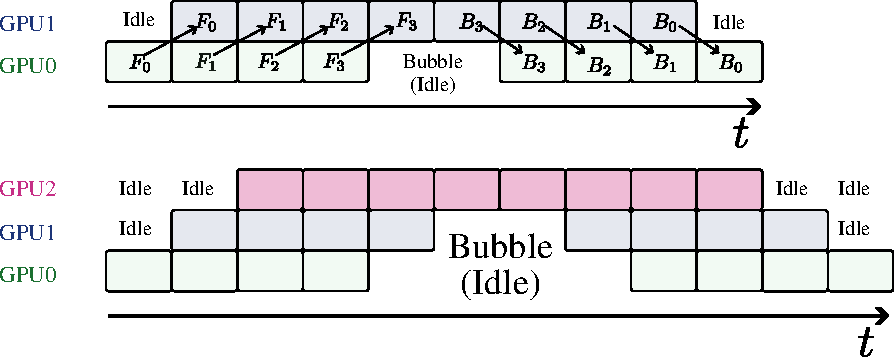
\includegraphics[scale=0.8]{./images/pipeline.pdf}
	\caption{The Illustration of the pipeline parallel on two GPUs. As you can see the bubble tends to grow as we increase the number of GPUs}
\end{figure}

\paragraph{Example:} Imagine a 2-stage pipeline parallel setup (for simplicity):

\begin{itemize}
	\item GPU 0: Holds Layers 1–3  
	\item GPU 1: Holds Layers 4–6  
\end{itemize}

If you have a batch of data with 32 samples, you might split it into 4 micro-batches of size 8 each. Then, forward Pass can be processed as follows:
\begin{enumerate}
	\item Micro-Batch 1
		\begin{enumerate}
			\item Step A: GPU 0 processes layers 1–3 for micro-batch #1.
			\item Step B: Once GPU 0 is done with those layers, it sends the activations for micro-batch #1 over to GPU 1.
			\item Step C: GPU 1 then processes layers 4–6 for micro-batch #1.
		\end{enumerate}
	\item Micro-Batch 2
		\begin{enumerate}
			\item As soon as GPU 0 finishes Step A for micro-batch #1 and passes the data to GPU 1, GPU 0 is free to start micro-batch #2 (layers 1–3).
			\item Meanwhile, GPU 1 is busy processing micro-batch #1 (layers 4–6).
			\item Once GPU 0 finishes its part for micro-batch #2, it sends those activations to GPU 1—which will be ready to handle them as soon as it’s done with micro-batch #1.
		\end{enumerate}
	\item Micro-Batch 3 and 4
		\begin{enumerate}
			\item This pattern continues in an overlapping fashion: while GPU 1 is busy with micro-batch #2, GPU 0 can start on micro-batch #3, and so on.
		\end{enumerate}
\end{enumerate}

The key benefit is concurrency:
\begin{itemize}
	\item While GPU 0 is processing micro-batch 2, GPU 1 can process micro-batch 1.  
	\item This overlap leads to higher GPU utilization.
\end{itemize}

Backward pass is a bit more complex because:
\begin{itemize}
	\item You need gradient signals to flow in the reverse order of the forward pipeline.  
	\item Each stage waits until it receives the gradient from the next stage before it can compute its own local gradients and pass them back to the previous stage.
\end{itemize}

However, the overall concept is similar-multiple stages can run backprop (on different micro-batches) in parallel, thereby keeping all GPUs busy.


\subsection{Pipeline Bubbles}

When using pipeline parallelism, you often hear about \textit{pipeline bubbles}. This refers to idle times on some GPUs before the assembly line is fully loaded or after it starts to wind down. 
\begin{itemize}
	\item Start-up Bubble: In the very beginning, GPU 1 must wait until GPU 0 finishes the first forward pass for micro-batch 1. GPU 1 sits idle during that initial delay.  
	\item Wind-down Bubble: After the last micro-batch enters GPU 0, GPU 1 continues to process the pipeline while GPU 0 is idle.
\end{itemize}

These bubbles can lead to less-than-ideal speedups, but you can mitigate them by using enough micro-batches to keep the pipeline busy most of the time.

\subsection{Combining Pipeline Parallelism with Other Forms of Parallelism}

In practice, pipeline parallelism is often combined with:
\begin{itemize}
	\item Data Parallelism: You still replicate each stage across multiple GPUs to handle separate shards of data.  
	\item Tensor Parallelism / Model Parallelism: Instead of giving entire layers to one GPU, you split the parameters or compute of a single layer across multiple GPUs (common in large language model setups, \eg Megatron-LM).  
	\item Sharded Optimizer Approaches (\eg ZeRO, FSDP): Distribute optimizer states and gradients to reduce memory overhead.
\end{itemize}


\section{1F1B}

\begin{figure}[t]
	\centering
	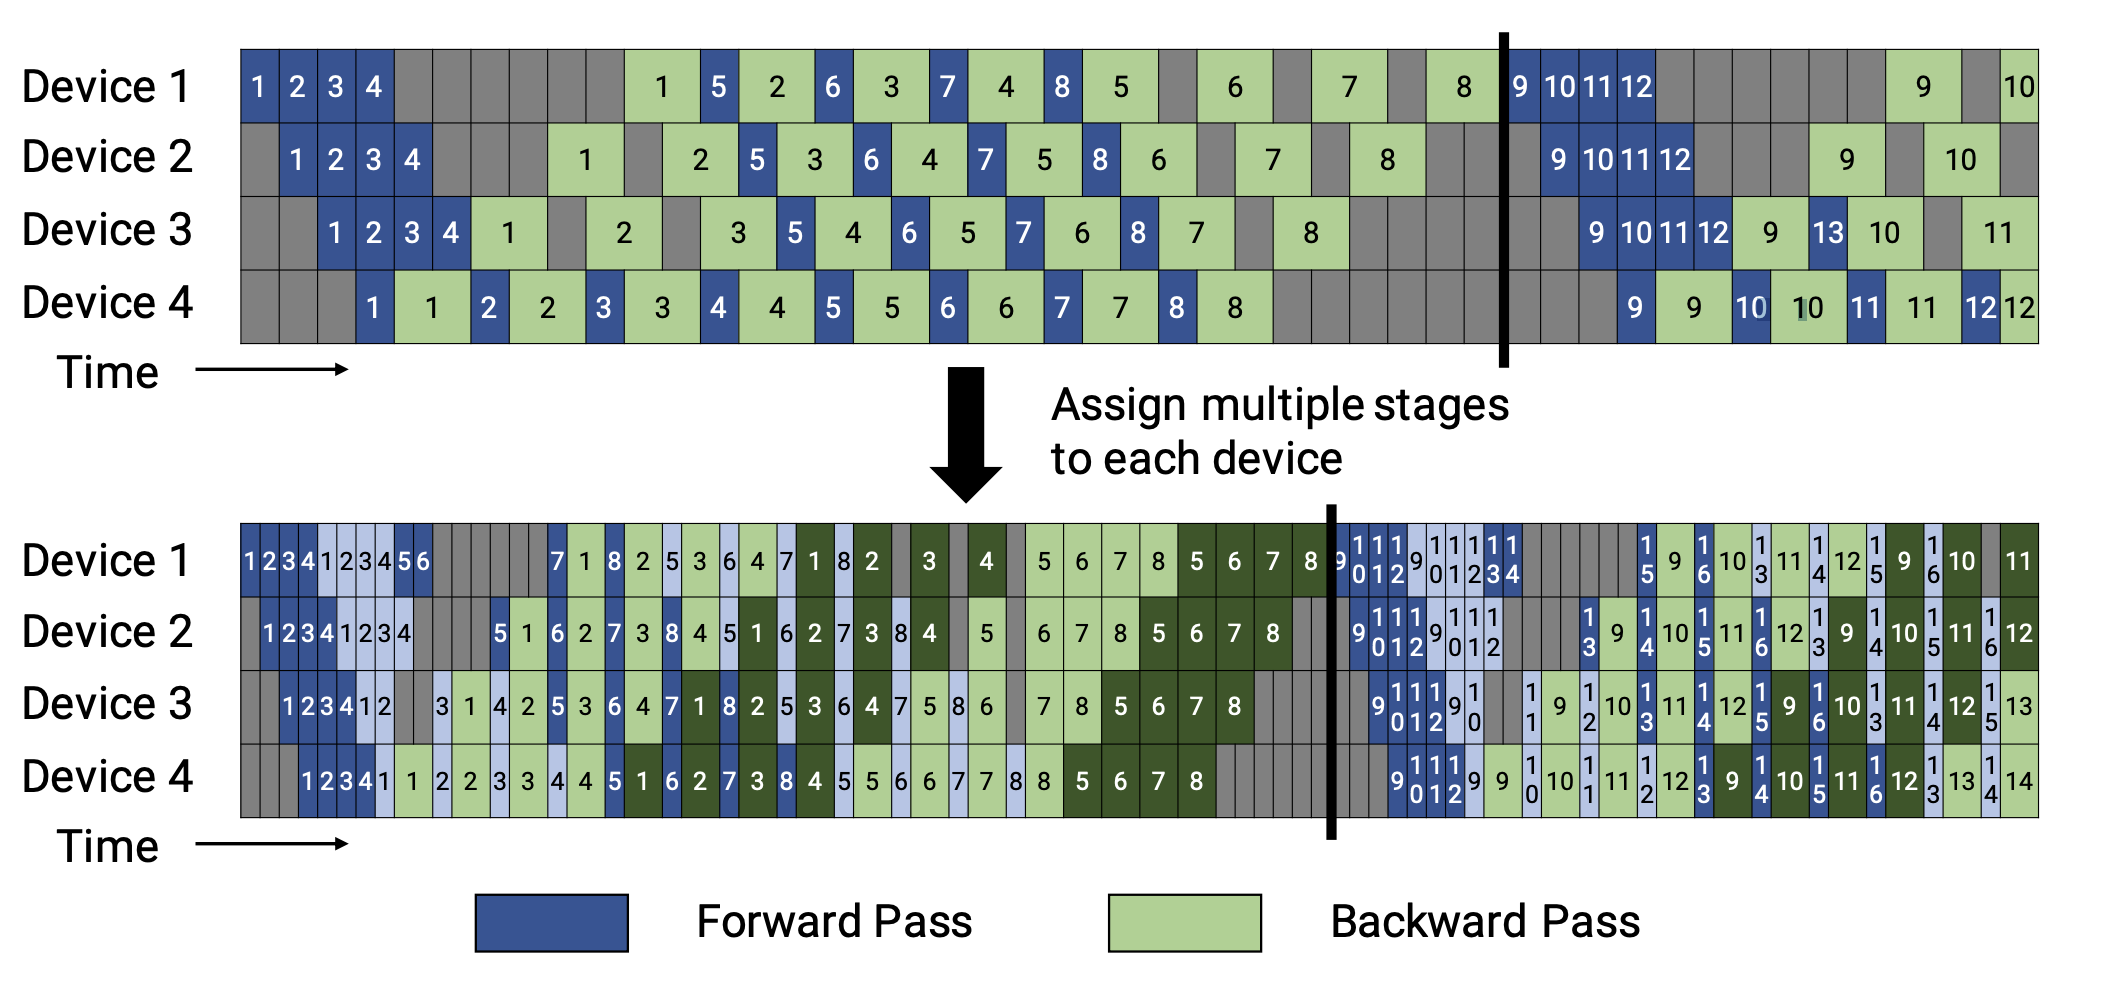
\includegraphics[scale=0.23]{./images/1f1b.png}
\end{figure}

\subsection{Non-interleaved Schedule}

The non-interleaved schedule can be divided into two states. The first state is the startup state (or warm-up state). In the startup state, After completing the forward pass for the first minibatch, it performs the backward pass for the same minibatch, and then starts alternating between performing forward and backward passes for subsequent minibatches. As the backward pass starts propagating to earlier stages in the pipeline, every stage starts alternating between forward and backward pass for different minibatches. As shown in the above figure, in the steady state, every machine is busy either doing the forward pass or backward pass for a minibatch.

\subsection{Interleaved Schedule}

This schedule requires the number of microbatches to be an integer multiple of the stage of pipeline. In this schedule, each device can perform computation for multiple subsets of layers(called a model chunk) instead of a single contiguous set of layers. \ie Before device 1 had layer 1-4; device 2 had layer 5-8; and so on. But now device 1 has layer 1,2,9,10; device 2 has layer 3,4,11,12; and so on. With this scheme, each device in the pipeline is assigned multiple pipeline stages and each pipeline stage has less computation. This mode is both memory-efficient and time-efficient.


\section{Zero Bubble}
\label{sec:}


\part{Compression}
\chapter{Model Compression}
\section{Introduction}
haha




\backmatter
% bibliography, glossary and index would go here.

\nocite{*}
\bibliographystyle{unsrt}
\bibliography{references}
\end{document}
